% Semantic Assistants - http://www.semanticsoftware.info/semantic-assistants
%
% This file is part of the Semantic Assistants architecture.
%
% Copyright (C) 2009, 2010, 2011, 2012 Semantic Software Lab, http://www.semanticsoftware.info
% The Semantic Assistants architecture is free software: you can
% redistribute and/or modify it under the terms of the GNU Affero General
% Public License as published by the Free Software Foundation, either
% version 3 of the License, or (at your option) any later version.
%  
% This program is distributed in the hope that it will be useful,
% but WITHOUT ANY WARRANTY; without even the implied warranty of
% MERCHANTABILITY or FITNESS FOR A PARTICULAR PURPOSE.  See the
% GNU Affero General Public License for more details.
% 
% You should have received a copy of the GNU Affero General Public License
% along with this program.  If not, see <http://www.gnu.org/licenses/>.


\chapter{OpenOffice/LibreOffice Writer Plug-In}
%TODO: update screenshots
The OpenOffice/LibreOffice application suite offers a mechanism
to add application extensions, or plug-ins. We used this
mechanism to integrate OpenOffice.org's word processing
application Writer with our architecture, and thus equip the
Writer with Semantic Assistants \citep{giwi08}.

Our primary goal for the Writer extension was to be able
to perform text analysis on the current document. This
text can, for instance, be a large document from which
information should be extracted, or a problem statement
consisting of a few questions, which serves as input for a
question-answering (QA) Semantic Assistant. Especially
for the last use case, it must allow a user to highlight part of
a document (e.g., a question) and be able to pass only the
highlighted part as input to a language service. Furthermore,
the extension must offer the possibility to specify parameters
that need to be passed to a selected NLP service.

An OpenOffice.org plug-in is basically a zip file with specific
contents and certain descriptions of these contents.  For a detailed
description of the implementation please refer to
Section~\ref{sec:oo-spec}. \textbf{Note:} The current version of the
plug-in requires at least OpenOffice.org Version 3.1.


\section{Features}
Our plug-in creates a new menu entry ``Semantic Assistants:''
\begin{center}
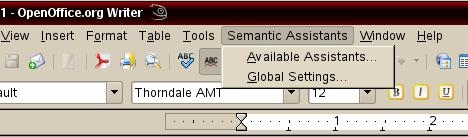
\includegraphics[width=0.7\textwidth]{pictures/oomenu.jpg}
\end{center}

In this menu, the user can inquire about available services, which are
selected based on the client (here \emph{Writer}) and the language
capabilities of the deployed NLP services (described in service
metadata, see Section~\ref{sec:owl}). The dynamically generated list
of available services is then presented to the user, together with a
brief description, in a separate window, as shown in
Figure~\ref{fig:oolist}. Note that the integration of a new service
does not require any changes on the client side---any new NLP service
created and deployed by a language engineer is dynamically discovered
through its OWL metadata maintained by the architecture and so becomes
immediately available to any connected client.
\begin{figure}[htb]
  \centering
  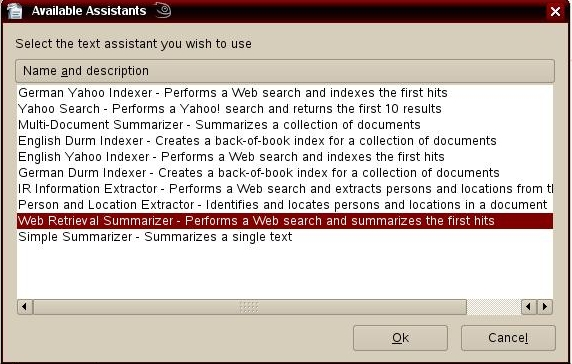
\includegraphics[width=0.5\textwidth]{pictures/oolist.jpg}
  \caption{List of available semantic assistants}
  \label{fig:oolist}
\end{figure}

The user can now select an assistant and execute it. In case the
service requires additional parameters, such as the length of a
summary to be generated, they are detected by our architecture through
the OWL-based service description and requested from the user through
an additional dialog window. An example, for the \emph{Web Retrieval
  Summarizer} assistant, is shown in Figure~\ref{fig:ooparams}.
\begin{figure}[htb]
  \centering
  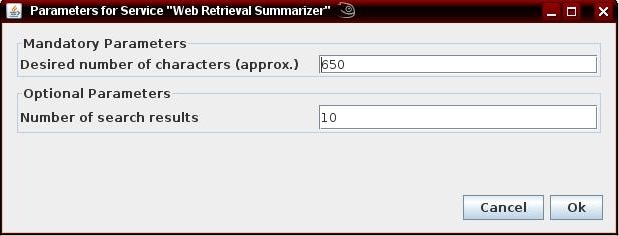
\includegraphics[width=0.5\textwidth]{pictures/ooparams.jpg}
  \caption{The parameters dialog, which appears when a Semantic
    Assistant requiring further input is invoked}
  \label{fig:ooparams}
\end{figure}
After the service is executed, the result is displayed in Writer depending on
the type of the server response: either as a new document, as annotations on
the existing document, or by opening an external viewer (e.g., a Web browser
for HTML documents).

\subsection{Side-Notes View}
The latest release of the OpenOffice.org Suite offer a new feature for text
annotation.  Depending on the annotation results received from GATE, the
Semantic Assistants Writer plug-in presents it in a sidenote manner (see
Figure~\ref{fig:sidenotes}).
\begin{figure}[htb]
  \centering
  %\vspace*{-9mm}
  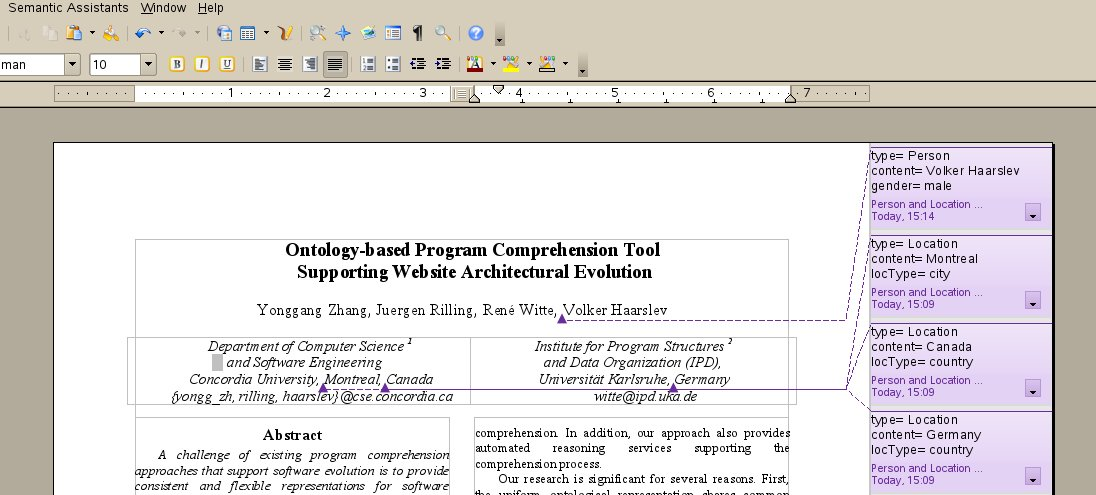
\includegraphics[width=0.8\textwidth]{pictures/sidenotes.jpg}
  \caption{Auto-Generated SideNotes Example}
  \label{fig:sidenotes}
  %\vspace*{-0.4cm}
\end{figure}

\subsection{New Document Creation}
\label{sec:doc-cre}
Creation of a new document comes handy when the output of an NLP service
corresponds to a complete document, or the result itself is indivisible. Some
examples are summarization or question-answering (see Figure~\ref{fig:oores}).

\begin{figure*}[htb]
  \centering
  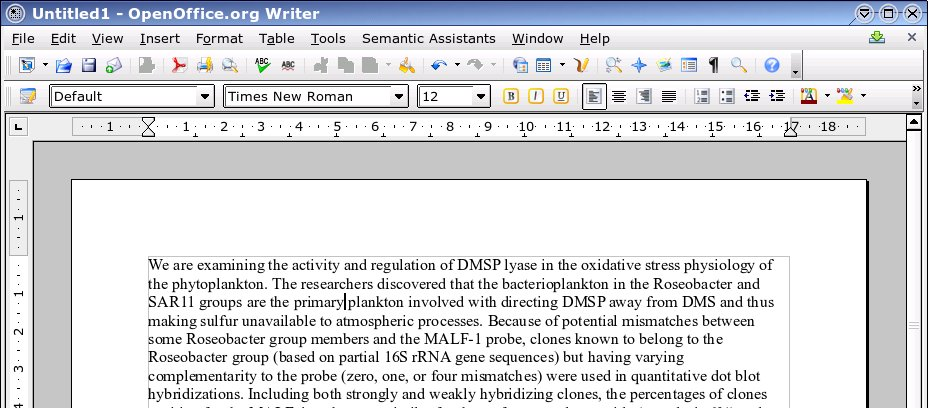
\includegraphics[width=0.8\textwidth]{pictures/ooresult_clip.jpg}
  \vspace*{-2mm}
  \caption{NLP services can also create a completely new document as a
  result (e.g., through summarization)}
  \label{fig:oores}
\end{figure*}

\subsection{Annotation Highlighting}
Besides text annotation, we offer the option for enabling/disabling annotation
highlighting for text that has been processed by GATE. This option can be
found under the Semantic Assistants menu in ``Global Settings.''  See
Figure~\ref{fig:highlight} for an example.

\subsection{Filter Empty Features}
This option found under the Semantic Assistants menu in ``Global Settings'' (shown
in Figure~\ref{fig:oosettings}) allows the ability to enable/disable filtering of
empty valued features in side-nodes. This can be useful to avoid cluttering or aid
debugging annotations respectively.

\subsection{Show Annotation Content}
This option in the ``Global Settings'' dialog can be used to include/exclude
the annotated content within the side-note. This can be used as an alternative
to annotation highlighting.

\begin{figure}
  \centering
  %\vspace*{-9mm}
  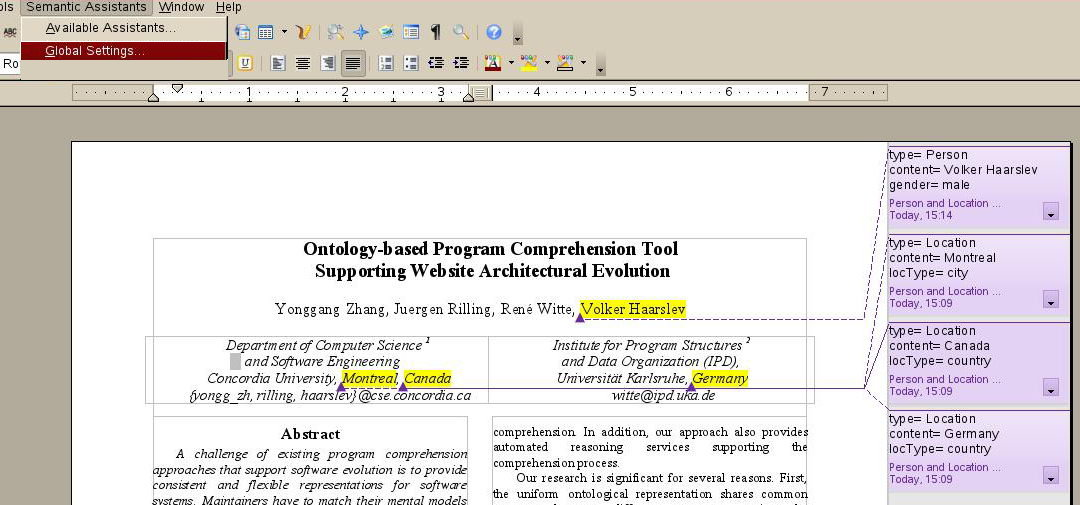
\includegraphics[width=0.8\textwidth]{pictures/highlighting.jpg}
  \caption{Highlighted Annotations Example}
  \label{fig:highlight}
  %\vspace*{0.5cm}
\end{figure}

\begin{figure}[htb]
\begin{center}
  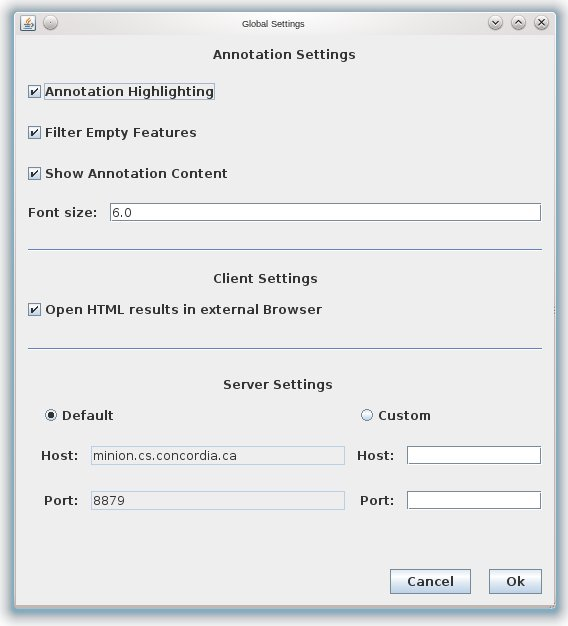
\includegraphics[width=0.5\textwidth]{pictures/oosettings.jpg}
  \caption{Configuration Dialog}
  \label{fig:oosettings}
\end{center}
\end{figure}

\subsection{Annotation Font Size}
As shown in Figure~\ref{fig:oosettings}, the font size of annotations can be changed
prior to invoking assistants. Due to the fixed width of side-notes, customizing the
size can ease readability of features.

\subsection{Browser Handling of HTML Results}
Instead of returning annotations, some pipelines produce HTML documents. The
``Open HTML results in external Browser'' option shown in Figure~\ref{fig:oosettings},
allows OpenOffice to invoke a local browser to display these results.

\subsection{Server Settings}
Another option found under the Semantic Assistants menu in ``Global
Settings.'' is \emph{Server Settings}.  There the user is able to specify the
Server information (Host and Port) of a local or distant server.

\section{Installation}
\label{subsec:oo-inst}
The OpenOffice.org plug-in can be found in
\url{SemanticAssistants/Clients/OpenOffice} and it is compatible with 
OpenOffice versions greater than 2.0.4. To use it, do the following:

\begin{enumerate}
  % TODO: what about the OO SDK installation? 
  % Is it needed for running the plug-in?

  \item Start OpenOffice.org Writer and ensure the right Java VM is
  used. Go to \emph{Tools $\rightarrow$ Options}. Under
  \emph{OpenOffice.org} you will find a \emph{Java} item. There, you
  can specify JREs. If it is not already there, add the currently used
  Java version.
  
  % should add screenshots for this
  \item Go to \emph{Tools $\rightarrow$ Extension Manager}. Click the
    \emph{Add$\ldots$} button on the bottom. Navigate to your local
    copy of the \sa\ architecture and then to
    \texttt{Clients/OpenOffice}. Select the file
    \texttt{SemassistOpenOfficePlugIn.oxt} and click \emph{Open}.

  \item Leave the dialog and open a new text document. You should have
    a new menu bar entry labeled \emph{Semantic Assistants}. Now you
    can run services on the current document (remember the server must
    be running to be able to query or execute language services).
\end{enumerate}


\section{Development Notes}
\label{sec:oo-spec}
In this section, we provide further technical details on our plug-in
for developers interesting in enhancing or modifying it.

\subsection{Compiling the Plug-in}
If you want to build the plugin yourself, follow these steps:
\begin{itemize}
  \item cd to the \url{Clients/OpenOffice} directory.

  \item Type \texttt{ant run}, or \texttt{ant run-gui}. Note that the
    client-side abstraction layer must have already been built and
    packaged. Both \texttt{ant run} and \texttt{ant run-gui} provide
    an UNO package named \url{SemassistOpenOfficePlugIn.oxt}. Both
    targets additionally copy it to \url{~/Documents/uno-components}.
    If \texttt{ant run-gui} is issued the OpenOffice.org
    \emph{Extension Manager} will pop up and prompt the user to
    install the extension.  If \texttt{ant run} is issued the above
    process is automated.  After the installation, OpenOffice Writer
    starts with the plug-in installed.

    \textbf{Note:} you can also manually add the plug-in from within
    OpenOffice (skip this step if you already used the \emph{run} or
    \emph{run-gui} target): Go to Tools, Extension Manager. Select
    \emph{My Extensions}, then click \emph{Add...} on the
    right. Choose the UNO package (available in
    \url{~/Documents/uno-components} if you used the \emph{deploy}
    target for ant).
\end{itemize}

\subsection{OpenOffice.org Plug-in Specifics}
Every plug-in has to include a \emph{description.xml} that describes the 
package's meta details like publisher, license, download url and version dependencies.
See \href{http://wiki.services.openoffice.org/wiki/Documentation/DevGuide/Extensions/Description_of_XML_Elements}{OpenOffice Developer's Guide}
for a list of available elements. The plug-in package also includes a
\emph{META-INF} directory, which contains a file called
\emph{manifest.xml}. This XML file lists the elements that come with
this plug-in;  The concrete manifest file for our plug-in is listed in
Figure~\ref{list:manifest}.  We can see that it defines three
\emph{file-entry} elements specifying the type and location of the
following files:
\begin{figure}[tb]
\centering
\begin{lstlisting}[language=XML,numbers=left,xleftmargin=8mm,columns=flexible]
<?xml version="1.0" encoding="UTF-8"?> 
<!DOCTYPE manifest:manifest PUBLIC 
"-//OpenOffice.org//DTD Manifest 1.0//EN" "Manifest.dtd"> 
<manifest:manifest 
 xmlns:manifest="http://openoffice.org/2001/manifest"> 
  <manifest:file-entry 
     manifest:media-type=
        "application/vnd.sun.star.configuration-data" 
     manifest:full-path="Addons.xcu"/> 
  <manifest:file-entry 
     manifest:media-type=
        "application/vnd.sun.star.configuration-data" 
     manifest:full-path="ProtocolHandler.xcu"/> 
  <manifest:file-entry 
     manifest:media-type=
        "application/vnd.sun.star.uno-component;type=Java" 
     manifest:full-path=
        "ProtocolHandlerAddon_java.uno.jar"/>
   <!-- Add any other plug-in required jar files here. -->
</manifest:manifest> 
\end{lstlisting}
\caption{The \emph{manifest.xml} file for our plug-in}
\label{list:manifest}
\end{figure}


\begin{description}
\item[\emph{Addons.xcu}.] This XML file defines how the plug-in should
  be integrated with OpenOffice.org. In our case, it contains a menu
  definition, specifying that the menu should only appear in the
  \emph{Writer} application. For each menu item, we specify which
  messages should be broadcast throughout the OpenOffice.org runtime
  system when the menu item is activated.
\item[\emph{ProtocolHandler.xcu}. ] This XML file specifies that the
  messages defined in \emph{Addons.xcu} should be handled by an object
  of a certain class. This class is provided in the Java archive and
  must adhere to a certain interface. 
\item[\emph{ProtocolHandlerAddon\_ java.uno.jar}.] This Java archive
  contains the actual functionality of the plug-in. It holds classes
  responsible for receiving the messages generated by the menu items,
  as well as classes responsible for the interaction with the
  client-side abstraction layer.
\end{description}


\subsection{Implementation Details}
A useful class called \url{UNOUtils} found in the \url{package
  info.semanticsoftware.semassist.client.openoffice.utils} contains most of
the OO-Writer feature implementations.  More specifically, the three methods in
Figure~\ref{list:ssb} implement a major part of the above described features
(Side-Notes, Highlighting and New Document Creation).

\begin{figure}
\centering
\begin{lstlisting}[language=Java,numbers=left,xleftmargin=8mm,columns=flexible]

private static XComponent CreateNewDocument( XDesktop xDesktop, 
					     String sDocumentType )
{
	...
}

private static void AnnotateField( Annotation annotation )
{
	...
	// Use the text document's factory to create an Annotation text field
	XTextField xAnnotation = (XTextField) UnoRuntime.queryInterface(
		XTextField.class, mxDocFactory.createInstance(
		"com.sun.star.text.TextField.Annotation" ) );
	
	// get the properties of the field
	XPropertySet xPropertySet = (XPropertySet) UnoRuntime.queryInterface( 
						XPropertySet.class, xAnnotation
);
	
	...
	
	// Highlight annotated field
        HighlightField();
}

private static void HighlightField()
{
....

}
\end{lstlisting}
\caption{Core methods implementing the OpenOffice Writer plug-in features are
  part of the \texttt{UNOUtils} class}
\label{list:ssb}
\end{figure}

%More details on how to compile and debug an OpenOffice plug-in can be found in Section~\ref{sec:debug}.
 
\subsection{Configure the OpenOffice Writer to Run in Debug Mode}
This Section describes how to configure the JAVA VM in OpenOffice Writer to accept incoming connection for a debugger.

\begin{enumerate}
  \item Open OpenOffice Writer
  \item Go to Tools, Options. Under \emph{OpenOffice.org}, there is a \emph{Java} item. Select it and then Click on the 
        \emph{Parameter} button. There the parameters when running the JAVA VM are set.
  \item To run in debug mode \emph{Assign} the following 2 parameters:
  \begin{itemize}
    \item \textbf{-X debug}
    \item \textbf{-Xrunjdwp:transport=dt\_socket,server=y,suspend=n,address=7081}
  \end{itemize}
  \item \textbf{Note: The} \emph{address=7081} \textbf{should be the consistent with the port set within the debugger}
  \item  Now OO Writer is ready to accept connections from the debugger
\end{enumerate} 
